\chapter{Iqbal Syarif Awalludin (1144095)}
\begin{figure}[!htbp]
  \centering
  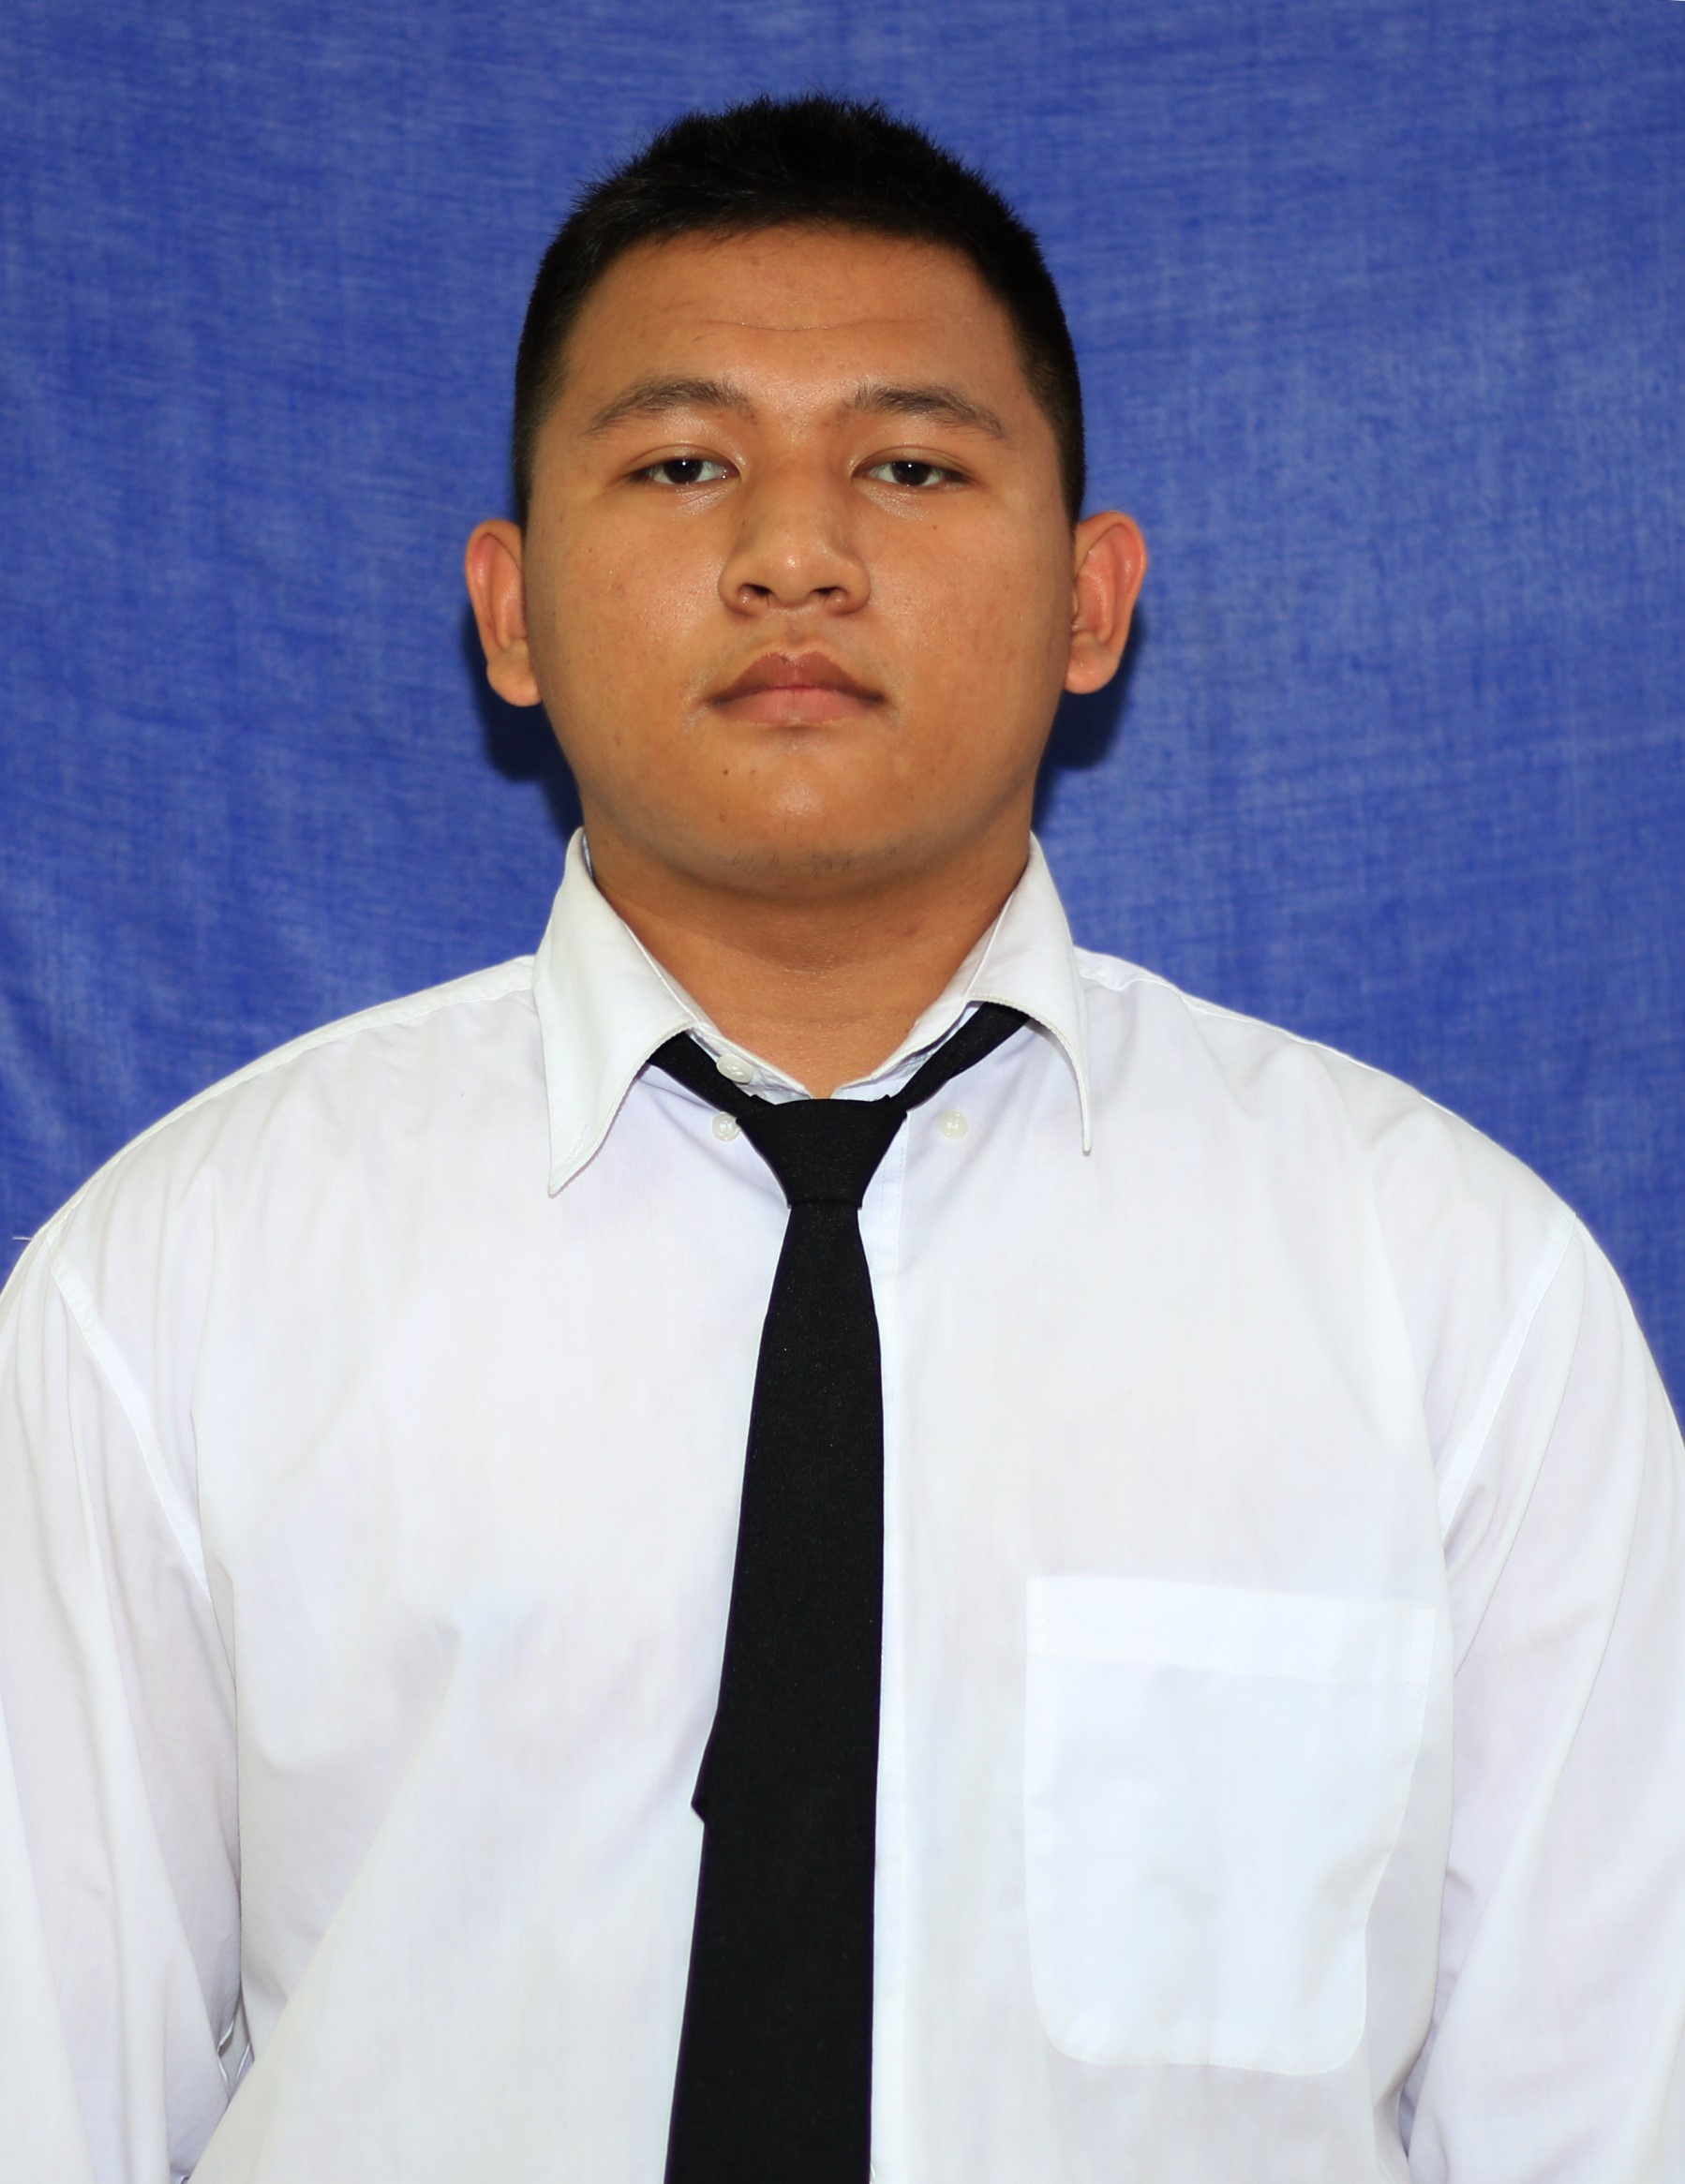
\includegraphics[width=.4\textwidth]{figures/Fotomhs/1144095.jpg}
  \caption{Ini adalah Iqbal Syarif Awaludin}\label{fig:1144095}
\end{figure}
Berikut adalah kegiatan Internship 2 di Prodi D4 Teknik Informatika tertera pada tabel \ref{table:kegiatanharian}
\begin{table}[!ht]
\centering
\begin{tabular}{ |c|c|c|c|c|c|c|c|c|c| }
\hline
No. & Judul Commit & Baris & Kode Commit & Tanggal \\
\hline
1 & Menambah materi macam2 sensor & (\#42) & 2f5ff92660a69b15c4ea4c4c1fd54a4dcdf02f83 & 25/02/2019 \\
\hline
2 & Membuat poster Sistem antrian dan menambah materi Arduino IDE & (\#43) & b9f90a23a64fba1616df40096016e833c9609e78 & 26/02/2019 \\
\hline
3 & Mengedit buku IOT khususnya bagian Software, Mengedit Laporan2019 khususnya rekomendasi kelulusan dan penilaian & (\#2) & ace406d89cdb4a64623650a1f3b4c8aa4e223635 & 27/02/2019 \\
\hline
\end{tabular}
\caption{Tabel Kegiatan Harian}
\label{table:kegiatanharian}
\end{table}
\subsection{28/02/2019}
\begin{enumerate}
  \item Evaluasi mingguan
  \item Koreksi Laporan Proyek 2 Mahasiswa
  \item Menambah materi installasi IDE pada Arkom2019 \#44
  https://github.com/BukuInformatika/Arkom2019/commit/e2c587aa9be2382dc0701bda0a4839f6556289ee
\end{enumerate}
